%======================================================================
\chapter{Hollow-Core Optical Waveguides}
%======================================================================
\section{Conventional TIR Fibers}
Conventional optical fibers (and optical waveguides in general) are guided by TIR. Structurally, this is composed of a high refractive-index core $n_2$ surrounded by a lower refractive-index cladding $n_1$, depicted in Fig.\ref{fig:tir}.
\begin{figure}[h]
	\centering
	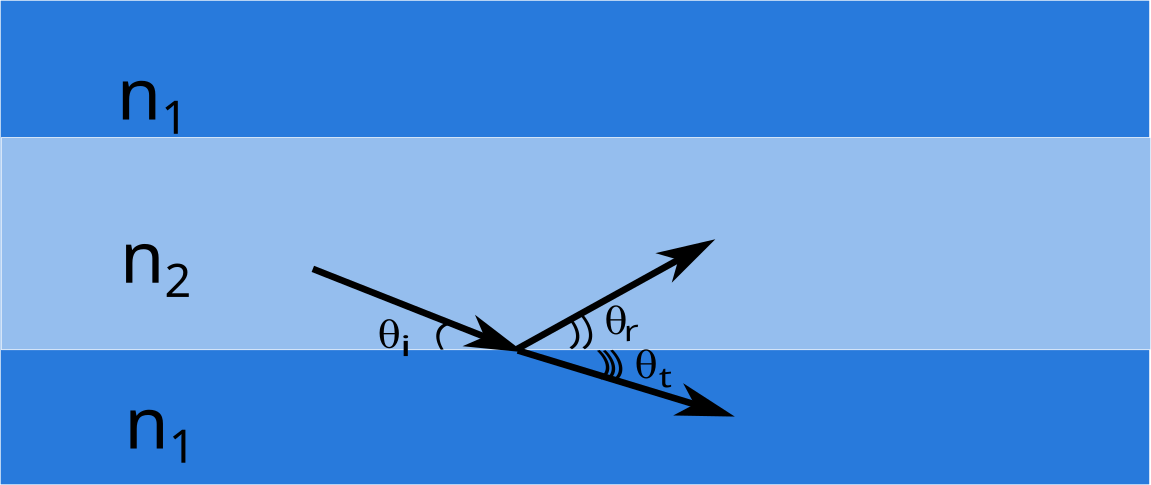
\includegraphics[width=0.6\textwidth]{./Figures/HCPCF/tir.png}
	\caption {Light propagation through optical fiber. The incident $\theta_i$, reflected $\theta_r$, and transmitted $\theta_t$ rays at the core-cladding boundary}
	\label{fig:tir}
\end{figure}
As light propagates through the the core, some light will be transmitted through the cladding while some is reflected back into the core. The relationship between the angles of incident and transmitted light is governed by Snell's Law:
\begin{equation}
	n_1cos(\theta_i) = n_2cos(\theta_t)
	\label{snell}
\end{equation}
If the refraction angle is at a minimum, then the light below a critical incident angle $\theta_{c}$, will not propagate into the cladding and will only be reflected back into the core, hence "total internal reflection". From Snell's law it is evident that the critical angle is dependent on the refractive-index contrast between the core and cladding, 
\begin{equation}
	\theta_c =arccos(n_2/n_1)
	\label{snell_crit}
\end{equation}
and that for TIR-guided fibers the core refractive index must be higher than that of the cladding otherwise light will just be transmitted through the cladding. The need for a higher core refractive index introduces limitations on the power transmission and intrinsic loss in TIR-guided fibers. 
\clearpage

\section{Photonic Crystal Bandgap}
The refractive-index contrast constraints of traditional fibers are overcome by HCPBFs which are able to mitigate the propagation losses in the core by having a core of air, $n_{air}=1$, the lowest possible refractive index. Light is instead trapped in the core by a photonic bandgap created by a surrounding photonic crystal cladding. 
\begin{figure}[htb!]
	\centering
	\begin{tabular}{cc}
		\multirow{-3}[15]{*}{\subfloat[]{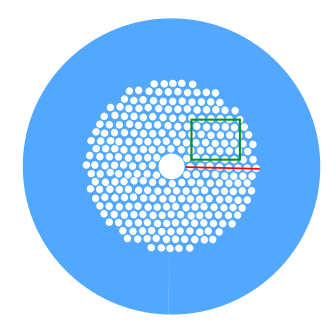
\includegraphics[width=7cm,height=7cm]{./Figures/HCPCF/HCPCF_section.png}}} &
		\subfloat[]{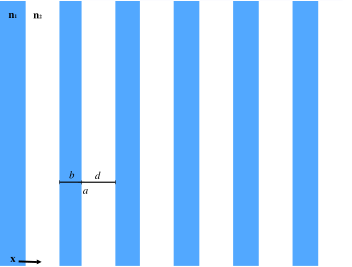
\includegraphics[width=4.5cm,height=3.5cm]{./Figures/HCPCF/HCPCF_1D.png}}                          \\&
		\subfloat[]{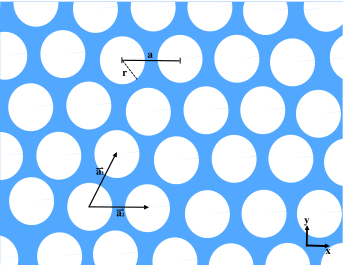
\includegraphics[width=4.5cm,height=3.5cm]{./Figures/HCPCF/HCPCF2D.png}}
	\end{tabular}
	\hfill
	\caption{(a)Cross-section a honey-comb HCPBF highlighting the PC pattern (b) Reduction of PC to 1-dimension (c)The 2-dimensional PC.}
	\label{fig:manyD}
\end{figure}
\clearpage
Photonic crystals consist of alternating refractive index in periodic structure, such a the 1D stack depicted in Fig.\ref{fig:manyD}(b) or 2D periodic array of air-holes seen in the HCPBF cross-section in Fig.\ref{fig:manyD}(c) . A periodic non-magnetic medium will have repeating dielectric constant \cite{yariv}
\begin{equation}
	\varepsilon(\boldsymbol{r}) = \varepsilon(\boldsymbol{r}+\boldsymbol{a})
\end{equation}
Due to its discrete and invariant translational symmetry, the dielectric constant along the medium can be expanded as the Fourier series
\begin{equation}
	\varepsilon(\boldsymbol{r}) = \sum_{\boldsymbol{G}}\varepsilon_{\boldsymbol{G}}e^{i\boldsymbol{G}\cdot\boldsymbol{r}}
	\label{eqn:fourier_eps}
\end{equation}
where $\boldsymbol{G}$ are the reciprocal lattice vectors such that $\boldsymbol{G}\cdot\boldsymbol{a} = 2\pi n$. The electric field can also be expressed as the Fourier integral
\begin{equation}
	\boldsymbol{E}(\boldsymbol{r}) = \iiint d^3\boldsymbol{k}\boldsymbol{A}(\boldsymbol{k})e^{i\boldsymbol{k}\cdot\boldsymbol{r}}
	\label{eqn:fourier_E}
\end{equation}
Using the Maxwell equations (\ref{eqn:maxwell}) the wave equation can be written in terms of the electric field
\begin{equation}
	\begin{aligned}
		\begin{cases}
			\vec{\nabla}\times\vec{H} & = -i\omega\epsilon(\vec{r})\vec{E} \\
			\vec{\nabla}\times\vec{E} & = i\omega\mu_0\vec{H}
		\end{cases}
	\end{aligned}
	\label{eqn:maxwell}
\end{equation}
\begin{equation}
	\boldsymbol{\nabla}\times(\boldsymbol{\nabla}\times\boldsymbol{E})-\omega^2\varepsilon(\boldsymbol{r})\mu_0\boldsymbol{E} = 0
\end{equation}
Substituting \eqref{eqn:fourier_eps} and \eqref{eqn:fourier_E} into the above equation results in the dispersion relation:
\begin{equation}
	\boldsymbol{k}\times(\boldsymbol{k}\times\boldsymbol{A}(\boldsymbol{k})) + \omega^2\mu_0\sum_{\boldsymbol{G}}\varepsilon_{\boldsymbol{G}}\boldsymbol{A}(\boldsymbol{k}-\boldsymbol{G}) = 0
	\label{eqn:separation}
\end{equation}
in where for any vector $\boldsymbol{K}$ the solutions of \eqref{eqn:separation} for the coefficient $\boldsymbol{A}(\boldsymbol{K})$ are grouped with the coefficients $\boldsymbol{A}(\boldsymbol{K}-\boldsymbol{G})$, decoupling the coefficients of other vectors that cannot be expressed in the form $\boldsymbol{K}-\boldsymbol{G}$. Disregarding the decoupled vectors, the total electric field can be described as a superposition of normal modes with regard to a chosen vector $\boldsymbol{K}$ :
\begin{equation}
	\boldsymbol{E}_{\boldsymbol{k}}(\boldsymbol{r}) = \sum_{\boldsymbol{G}}\boldsymbol{A}(\boldsymbol{K}-\boldsymbol{G})e^{i(\boldsymbol{k}-\boldsymbol{G})\cdot \boldsymbol{r}}
	\label{eqn:normalmodes}
\end{equation}
The Bloch theorem for the electric field can be pulled out  from \eqref{eqn:normalmodes}
\begin{equation}
	\boldsymbol{E}_{\boldsymbol{k}}(\boldsymbol{r}+\boldsymbol{a}) = e^{i\boldsymbol{k}\cdot \boldsymbol{a}}\boldsymbol{E}_{\boldsymbol{k}}(\boldsymbol{r})
\end{equation}
\begin{equation}
	\boldsymbol{u_k}(\boldsymbol{r}) = \sum_{\boldsymbol{G}}\varepsilon_{\boldsymbol{G}}e^{i\boldsymbol{G}\cdot\boldsymbol{r}}
\end{equation}
\begin{equation}
	\varepsilon_{\boldsymbol{G}} = \frac{1}{V}\int d^3\boldsymbol{r}e^{-i\boldsymbol{G}\cdot\boldsymbol{r}}\boldsymbol{u_k}(\boldsymbol{r})
	\label{eqn:perm}
\end{equation}
Returning to \eqref{eqn:separation}, can fix $\omega$ to find the corresponding $\boldsymbol{K}$ and normal modes os the system. However, in the case of photonic crystals there are ranges of frequencies that  have no $\boldsymbol{K}$s with real solutions, which implies that waves of these frequencies cannot propagate through the photonic crystal. These non-propagating frequencies are referred to as the photonic band gap.

\subsection{1D Photonic Bandgap}
1D photonic bandgap structure models for hollow-core optical fibers \cite{chourasia} demonstrate the core idea of bandgap fibers. In one dimension, the periodicity of dielectric constant is described by $\varepsilon(z) = \varepsilon(z+a)$ where $a = b+d$, the length of one period. The reciprocal lattice vector will be $\boldsymbol{G}_n = n\frac{2\pi}{a}\hat{z}$ and plugging into the Fourier series expansion of $\varepsilon(z)$  from \eqref{eqn:fourier_eps}
\begin{equation}
	\varepsilon(z)  =\sum_{n=-\infty}^\infty\varepsilon_ne^{in\frac{2\pi}{a}\hat{z}}
\end{equation}
From the reduction to propagation in the z-direction with the electric field oriented in x-direction, \eqref{eqn:separation} simplifies to
\begin{equation}
	K^2A(K) + \omega^2\mu_0\sum_{n=-i\infty}^\infty\varepsilon_nA(K-n\frac{2\pi}{a}) = 0
\end{equation}
Expanding the Fourier coefficients to the 1st order and reducing the equations to the dominant coefficients of the form $A(K)$ and $A(K-\frac{2\pi}{a})$ . $|K - g| = K$ and $K = \frac{\pi}{a}$ gives a system of equations that can be solved to find the dispersion relation $\omega(K)$.
\begin{equation}
	\begin{cases}
		\big(K^2-\omega^2\mu_0\varepsilon_{00}\big)A(K) = \omega^2\mu_0\varepsilon_1A(K - g) \\
		\omega^2\mu_0\varepsilon_{-1}A(K) = \big((K-g)^2-\omega^2\mu_0\varepsilon_{00}\big)A(K-g)
	\end{cases}
\end{equation}
The equations relating these two modes have a solution at
\begin{equation}
	\big(K^2-\omega^2\mu_0\varepsilon_{00}\big)\big((K-g)^2-\omega^2\mu_0\varepsilon_{00}\big) -\big(\omega^2\mu_0\varepsilon_1\big)\big(\omega^2\mu_0\varepsilon_{-1}\big)  = 0
\end{equation}
Noting that $\varepsilon_1 = \varepsilon_{-1}^*$ and $K\approx2g$ simplifies the relationship to
\begin{equation}
	\omega_{\pm}^2 = \frac{K^2}{\mu_0(\varepsilon_{00}\mp|\varepsilon_1|)}
\end{equation}
The dispersion relation has two possible solutions, which specify the top and bottom of the photonic bandgap edges, as illustrated in Fig.\ref{fig:1dbp}.
\begin{figure}[h]
	\centering
	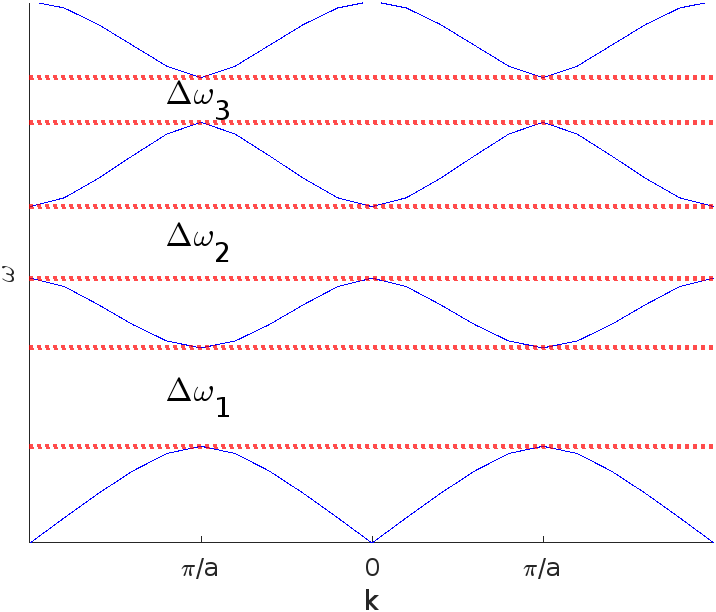
\includegraphics[width=0.6\textwidth]{./Figures/HCPCF/1D_BandGap.png}
	\caption {Band plot for a 1D photonic crystal with parameters-,-, solved using Finite Difference Time Domain(FDTD) method\cite{sukhoivanov}.}
	\label{fig:1dbp}
\end{figure}

If solving for the wavevector at a frequency between the two roots $\omega_{\pm}$, only complex solutions will exist. This means that only evanescent waves, not electromagnetic waves, propagate through the medium while the electromagnetic waves are reflected back; the medium acts as a mirror for the bandgap wavelengths.\\
This is the phenomenon that allows for HCPBF to guide certain frequencies of light: wavelengths in the bandgap are reflected by surrounding Bragg Grating confining them to the core of the fiber, while the rest are allowed to propagate through the grating. 

\subsection{2D Photonic Bandgap}
To understand the full picture of light propagation in hollow-core fiber, the expansion to the 2D case pictured in Fig.\ref{fig:manyD}c is needed. However, with the electromagnetic waves now propagating in two dimension there is an added layer of complexity with the TE TM wave polarizations and the bandgaps. In addition to controlling the refractive index of the material and the period of the lattice, the lattice structure and hole radius will affect the performance of the photonic crystal, the latter playing a large role in the completeness of the photonic bandgap. In the 2D photonic crystal, the in-plane guided modes will have either magnetic fields in-plane and electric fields perpendicular to the lattice (TE modes), or electric fields in-plane and magnetic fields perpendicular to the lattice (TM modes). As the TE and TM modes are perpendicular to each other they may exhibit wildly different dispersion relations, which means that an optical bandgap is not guaranteed to persist for all polarizations\cite{joannopoulos}. This is certainly the case for square lattice phonic crystals, but other patterns such as the honeycomb (which is the structure in our HCPBF) have a bandgap persisting for all polarizations\cite{villeneuve}. It is important to consider all polarization effects when making decisions about photonic crystal patterns for two or more dimensions. \\
\begin{figure}[h]
	\centering
	\foreach \x in {HCPCF_2D_cartesian, HCPCF_2D_reciprocal}
		{
			\begin{subfigure}[b]{0.45\textwidth}
				\includegraphics[width=\textwidth]{./Figures/HCPCF/\x.png}
				\caption{}
			\end{subfigure}
			\hfil
		}
	\caption {(a) primitive lattice vectors and (b) primitive reciprocal lattice vectors with first Brillouin zone (green) and irreducible  Brillouin  zone (red) depicted for a honeycomb lattice structure.  }
	\label{fig:2d}
\end{figure}
\clearpage
Considering the lattice structure in Fig.\ref{fig:2d}(a) and taking propagation in the xy-plane ($K_z=0$ and $z=0$ for simplicity), the wavevector and position vectors reduce to  $\boldsymbol{K_{||}}=k_x\hat{x}+k_y\hat{y}$ and $\boldsymbol{r_{||}}=x\hat{x}+y\hat{y}$.  The primitive lattice vectors of a honeycomb photonic crystal will be:
\begin{equation}
	\boldsymbol{a}_1 = a\hat{x} \hspace{1cm} \boldsymbol{a}_2 = \frac{a}{2}\hat{x}+\frac{a\sqrt{3}}{2}\hat{y}
\end{equation}
and transforming to the momentum-space,  $\boldsymbol{b}\cdot\boldsymbol{a} = 2\pi\delta_{ij}$, as shown in Fig.\ref{fig:2d}(b) the primitive reciprocal lattice vectors are
\begin{equation}
	\boldsymbol{b}_1 = \frac{2\pi}{a}\hat{x}-\frac{2\pi}{a\sqrt{3}}\hat{y} \hspace{1cm} \boldsymbol{b}_2 =\frac{4\pi}{a\sqrt{3}}\hat{y}
\end{equation}
Taking these in combination of $n, m$ integer scaling factors, the reciprocal lattice vector is defined $\boldsymbol{G_{||}} = n\boldsymbol{b}_1 + m\boldsymbol{b}_2$.
The electromagnetic field defined for a two dimensional system is
\begin{equation}
	\boldsymbol{E}(\boldsymbol{r}) = e^{i\boldsymbol{k}\cdot\boldsymbol{r}}
	\sum_{m=-\infty}^\infty\sum_{n=-\infty}^\infty\boldsymbol{E}_{m,n}
	e^{i(n\boldsymbol{b_1}+m\boldsymbol{b_2})\cdot\boldsymbol{r}}
	\label{eqn:2d_emf}
\end{equation}
and the correlating Fourier expansion of dielectric function \eqref{eqn:perm}
\begin{equation}
	\varepsilon_{\boldsymbol{G_{||}}} = \frac{1}{a'\cdot b'}\int dxdye^{i(G_xx + G_yy)}\boldsymbol{u_k}(x, y)
	\label{eqn:2d_perm}
\end{equation}
are substituted into \eqref{eqn:maxwell}.
By utilizing the lattice symmetry and periodicity, the problem can be restricted to only solve for Bloch modes inside the of the irreducible Brillouin zone.
The first Brillouin zone is defined by the perpendicular bisectors to the primitive reciprocal lattice vectors, depicted in green in Fig.\ref{fig:2d}(b) and can be further subdivided into the irreducible Brillouin zone shown in red.
In order to find the photonic bandgap, solving the dispersion equation just along the irreducible Brillouin zone is sufficient.
For a honeycomb lattice, the $k$-path to follow would be
\begin{equation}
	\begin{cases}
		|\Gamma X| = \frac{2\pi}{a\sqrt{3}}, & k_x=0, 0<k_y<\frac{2\pi}{\sqrt{3}a}               \\
		|XJ| =  \frac{2\pi}{3a},             & 0<k_x<\frac{2\pi}{3a}, k_y=\frac{2\pi}{\sqrt{3}a} \\
		|\Gamma J| = \frac{4\pi}{3a},        & 0<k_x<\frac{2\pi}{3a}, k_y=\sqrt{3}k_x
	\end{cases}
\end{equation}
Discretizing  (\ref{eqn:2d_emf}) and (\ref{eqn:2d_perm}) then picking a few points along the $k$-path, numerical methods can be used to solve for the optical bandgap. Fig.\ref{fig:2dbp} shows the resulting TE bandgap for a honeycomb lattice with parameters $\varepsilon=11$,$\frac{r}{a}=0.34$, $a=3.8\mu$m using Plane Wave Expansion(PWE)\cite{sukhoivanov}.
\begin{figure}[h]
	\centering
	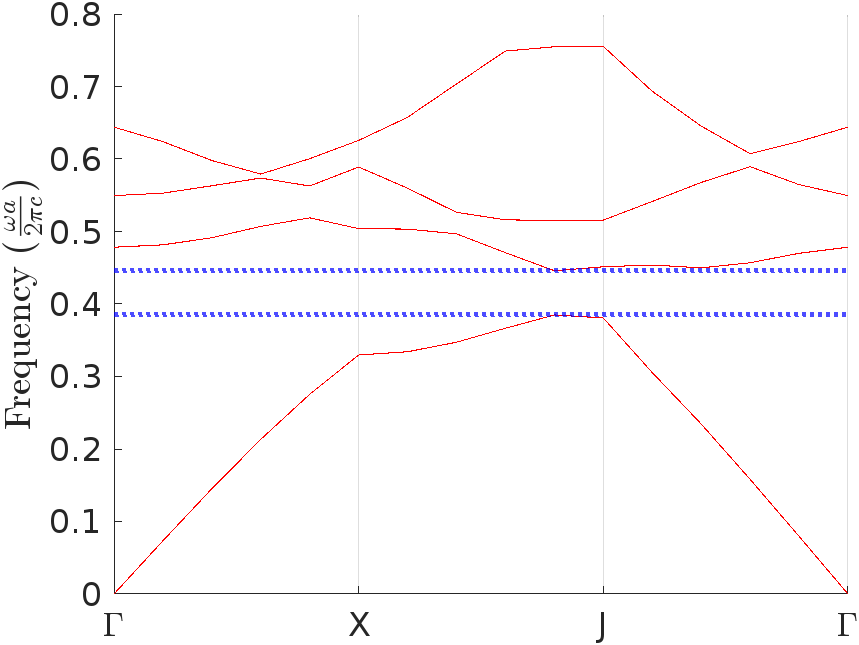
\includegraphics[width=0.8\textwidth]{./Figures/HCPCF/2D_BandDiagram.png}
	\caption {Band plot along the irreducible Brillouin zone for a honeycomb lattice with parameters $\varepsilon=11$,$\frac{r}{a}=0.34$, $a=3.8\mu$m. Solved by using the Plane Wave Expansion(PWE) numerical method.}
	\label{fig:2dbp}
\end{figure}
\clearpage
\subsection{Bandgap Shift}
The position of the HCPBF bandgap is dependent on the periodicity refractive-index and changing the material within the photonic crystal will cause a change in the bandgap. Though a small index contrast in the a periodic medium is assumed in the derivation, the bandgap shift has been experimentally confirmed to still hold under high contrasts\cite{antonopoulos}. The scalar wave equation for a given periodic medium will maintain the same bandgap structure but scaling the wavelength proportionately in compensation\cite{birks}. The scaling law for the wave equation for the transverse coordinates
$X=x\Lambda^{-1}$ $Y=y\Lambda^{-1}$
where $\Lambda$ is a solution to the transverse scale.
\begin{equation}
	n(X, Y) = \begin{cases}
		1, & n_1 \text{   (high RI)} \\
		0, & n_2 \text{   (low RI)}
	\end{cases}
\end{equation}
and factors into the normalized scaled wave equation:
\begin{equation}
	\nabla_\perp^2\Psi + (v^2n(X, Y) - w^2)\Psi = 0
\end{equation}
With $\nabla_\perp = \partial^2/\partial X^2 + \partial^2/\partial Y^2 $
solving for the frequency parameter $v^2$ and eigenvalue $w^2$:
\begin{equation}
	\begin{aligned}
		v^2 & = \Lambda^2k^2(n_1^2 - n_2^2)   \\
		w^2 & = \Lambda^2(\beta^2 - k^2n_2^2)
	\end{aligned}
\end{equation}
From the equation above it is evident that the eigenvalue is determined by the frequency parameter and the index distribution function $n(X, Y)$. This implies that $w^2$ and $v^2$ are invariant with changes to the parameters $k = \omega/c, \Lambda, n_1, n_2$.
In the HCPBF case where the glass refractive index is held constant and the air in the fiber is replaced by a new material. The equations can be rewritten with $n_1 = n_{glass}$ and $n_2 = n_{air}=1$:
\begin{equation}
	\begin{aligned}
		v^2 - w^2 & = \Lambda^2(k^2n_{glass} - \beta^2)                          \\
		v         & = k\Lambda n_{glass}\sqrt{n_{air} - \frac{n_{air}}{n_{new}}}
	\end{aligned}
\end{equation}
The initial index contrast $N_0 = \frac{n_{air}}{n_{glass}}$ moves to $ N = \frac{n_{new}}{n_{glass}}$ with the change in RI $n_{air} <  n_{new} < n_{glass}$. This leads to the new center bandgap to be governed by the equation:
\begin{equation}
	\lambda = \lambda_0\sqrt{\frac{1-N^{-2}}{1-N_0^{-2}}}
\end{equation}
\clearpage




